% Authors: Taejin Hwang
% Emails: taejin@berkeley.edu

\qns{System Identification}

In this question, we will take a look at how to \textbf{identify} a system by taking experimental data taken from a (presumably) linear system to learn a discrete-time linear model for it using the least-squares.

Recall that a \textbf{linear, continuous-time,} system can be put in state-space form:
\begin{equation}
\ddt{}{t} \vec{x}(t) = A \vec{x}(t) + \vec{b} u(t)
\end{equation}

Now let's say we have an \textbf{unknown} linear system in which we can give an input $u(t)$ and observe the output $\vec{x}(t).$ We can model the system using the following diagram:
\begin{center}
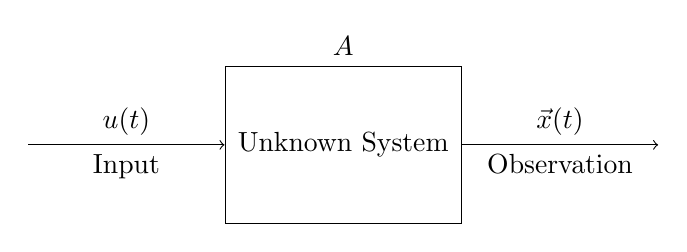
\begin{tikzpicture}
\node[draw, rectangle, minimum width = 3 cm, minimum height = 2 cm] (fl) at (0,0) {Unknown System};
\node[above] at (fl.north) {$A$};
\draw[<-] (fl) -- node[above]{$u(t)$} node[below]{Input} ++(-4,0);
\draw[->] (fl) -- node[above]{$\vec{x}(t)$} node[below]{Observation} ++(4,0);
\end{tikzpicture}
\end{center}

Recall from discussion that if we put a \textbf{piecewise constant} input $u(t) = u[n]$ for $t \in [nT, (n+1)T)$, where $T$ is the interval between samples, then we can observe the output $\vec{x}(t)$ at the $(n+1)^\text{th}$ time step and form a discretized model of the observation.

\begin{center}
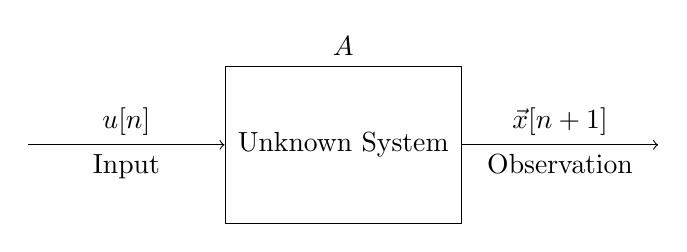
\begin{tikzpicture}
\node[draw, rectangle, minimum width = 3 cm, minimum height = 2 cm] (fl) at (0,0) {Unknown System};
\node[above] at (fl.north) {$A$};
\draw[<-] (fl) -- node[above]{$u[n]$} node[below]{Input} ++(-4,0);
\draw[->] (fl) -- node[above]{$\vec{x}[n + 1]$} node[below]{Observation} ++(4,0);
\end{tikzpicture}
\end{center}

\textbf{If} we knew the system, the relationship for between $\vec{x}[n+1], \ \vec{x}[n], $ and $u[n]$ would be:
\begin{equation}
\vec{x}[n + 1] = A \vec{x}[n] + \vec{b} u[n]
\end{equation}

While this relation is useful, we currently do not know what the $A$ matrix or $\vec{b}$ vector are. \textbf{The goal of system identification is to find $A$ and $\vec{b}$ from data to determine the dynamics of the system.}

For the purposes of this question, our state space will be $\mathbb{R}^2.$ \vskip 1pt
Therefore, we will start by creating unknown variables for the $A$ matrix, and $\vec{b}$ vector:
\begin{equation}
A = \begin{bmatrix} a_{11} & a_{12} \\ a_{21} & a_{22} \end{bmatrix} \ \ \text{and} \ \ \vec{b} = \begin{bmatrix} b_{1} \\ b_{2} \end{bmatrix}
\end{equation}

\begin{enumerate}
  \qitem Let's say the system initially started at $\vec{x}[0] = \begin{bmatrix} x_{1}[0] \\ x_{2}[0] \end{bmatrix},$ and we gave an input at time $t = 0, \ u[0].$ 
  At time $t = 1,$ we observe $\vec{x}(1) = \begin{bmatrix} x_{1}[1] \\ x_{2}[1] \end{bmatrix}.$
  
  \textbf{How can you uncouple this matrix/vector equation into a system of linear equations?}
  Hint: What are the unknowns that you are solving for?

  \ws {
    \vspace{75px}
  }

  \sol {
    We start by writing out the matrix/vector equation for our unknown system:
    \begin{equation}
    \vec{x}(1) = \begin{bmatrix} x_{1}(1) \\ x_{2}(1) \end{bmatrix} = A \vec{x}(0) + \vec{b} u(0) = 
    \begin{bmatrix} a_{11} & a_{12} \\ a_{21} & a_{22} \end{bmatrix} \begin{bmatrix} x_{1}(0) \\ x_{2}(0) \end{bmatrix} + 
    \begin{bmatrix} b_{1} \\ b_{2} \end{bmatrix} u(0)
    \end{equation}

    Uncoupling these equations, we get:
    \pagebreak[0]
    \begin{gather*}
    x_{1}(1) = a_{11} x_{1}(0) + a_{12} x_{2}(0) + b_{1} u(0) \\
    x_{2}(1) = a_{21} x_{1}(0) + a_{22} x_{2}(0) + b_{2} u(0)
    \end{gather*}
  }

  \qitem Based on the system of linear equations created in the previous part, \textbf{how many unknown} variables do we have? Also, if we have a system of linear equations with $n$ unknown variables, at the minimum, \textbf{how many equations} would we need to solve our system?

  \ws {
    \vspace{75px}
  }
  \sol {
    The unknowns in this system of linear equations are: $a_{11}, a_{12}, a_{21}, a_{22}, b_{1}, b_{2}.$ \vskip 1pt
    If we have a system of linear equations with $n$ unknown variables, we will need at least $n$ equations to solve the system. 
  }

  \qitem We now give another input at $t = 1, \ u[1],$ and observe the resulting state after one more time step $\vec{x}[2].$ \vskip 1pt 
  \textbf{How many more equations do we get from this observation? How many more observations will we need to make until we have enough equations?}

  \ws {
      \vspace{50px}
  }
  \sol {
    We can write out a similar observation as the one made in part(a):
    \begin{equation}
    \vec{x}(2) = \begin{bmatrix} x_{1}(2) \\ x_{2}(2) \end{bmatrix} = A \vec{x}(1) + \vec{b} u(1) = 
    \begin{bmatrix} a_{11} & a_{12} \\ a_{21} & a_{22} \end{bmatrix} \begin{bmatrix} x_{1}(1) \\ x_{2}(1) \end{bmatrix} + 
    \begin{bmatrix} b_{1} \\ b_{2} \end{bmatrix} u(1)
    \end{equation}

    Uncoupling these equations again, we will get:
    \pagebreak[0]
    \begin{gather*}
    x_{1}(2) = a_{11} x_{1}(1) + a_{12} x_{2}(1) + b_{1} u(1) \\
    x_{2}(2) = a_{21} x_{1}(1) + a_{22} x_{2}(1) + b_{2} u(1)
    \end{gather*}
    Notice that for every observation we make at a given time step, we will get $2$ more equations. 
    Taking the initial condition $\vec{x}(0)$ into account, we will have to make $4$ observations total, to get $6$ equations.
    In other words, we will have to start observing $\vec{x}(0)$ and continue up until $\vec{x}(3),$ to solve our system.
  }

  \qitem Assume we have collected all of the necessary measurements of $x[n]$ at time $n = 0, 1, 2, \ldots$ by letting the system run its course and recording the state variables at each time step. \vskip 1pt
  \textbf{How can we set up our system of linear equations as a matrix-vector equation?}

  \ws {
    \vspace{75px}
  }
  \sol {
    We can set up the following system of linear equations:
    $$
    \begin{bmatrix}
    x_{1}(0) & x_{2}(0) & u(0) & 0 & 0 & 0 \\
    x_{1}(1) & x_{2}(1) & u(1) & 0 & 0 & 0 \\
    x_{1}(2) & x_{2}(2) & u(2) & 0 & 0 & 0 \\
    0 & 0 & 0 & x_{1}(0) & x_{2}(0) & u(0) \\
    0 & 0 & 0 & x_{1}(1) & x_{2}(1) & u(1) \\
    0 & 0 & 0 & x_{1}(2) & x_{2}(2) & u(2) 
    \end{bmatrix} 
    \begin{bmatrix} a_{11} \\ a_{12} \\ b_{1} \\ a_{21} \\ a_{22} \\ b_{2} \end{bmatrix}
    = \begin{bmatrix} x_{1}(1) \\ x_{1}(2) \\ x_{1}(3) \\ x_{2}(1) \\ x_{2}(2) \\ x_{2}(3) \end{bmatrix}$$
    This can be written in as a matrix vector equation $D \vec{s} = \vec{y}$ and we can solve for $\vec{s} = D^{-1} \vec{y}$  
  }

  \qitem While we can set up a matrix vector equation and uniquely solve our system, the output of the system can be noisy.
  Therefore, we update our model by considering a noise term $w[n]$ at time $t = nT.$
  \begin{equation}
    \vec{x}[n + 1] = A \vec{x}[n] + \vec{b} u[n] + w[n]
  \end{equation}
  \textbf{How can we set up a system of equations in a similar fashion but with a noise vector $\vec{w}$?}

  \begin{equation}
    \vec{y} = D \vec{s} + \vec{w}
  \end{equation}

  \ws {
    \vspace{75px}
  }
  \sol {
    $$
    \begin{bmatrix} x_{1}(1) \\ x_{1}(2) \\ x_{1}(3) \\ x_{2}(1) \\ x_{2}(2) \\ x_{2}(3) \end{bmatrix} 
    = 
    \begin{bmatrix}
    x_{1}(0) & x_{2}(0) & u(0) & 0 & 0 & 0 \\
    x_{1}(1) & x_{2}(1) & u(1) & 0 & 0 & 0 \\
    x_{1}(2) & x_{2}(2) & u(2) & 0 & 0 & 0 \\
    0 & 0 & 0 & x_{1}(0) & x_{2}(0) & u(0) \\
    0 & 0 & 0 & x_{1}(1) & x_{2}(1) & u(1) \\
    0 & 0 & 0 & x_{1}(2) & x_{2}(2) & u(2) 
    \end{bmatrix} 
    \begin{bmatrix} a_{11} \\ a_{12} \\ b_{1} \\ a_{21} \\ a_{22} \\ b_{2} \end{bmatrix}
    + \begin{bmatrix} w(0) \\ w(1) \\ w(2) \\ w(0) \\ w(1) \\ w(2) \end{bmatrix} $$
  }

  \qitem We can try to solve our system of equations, but we do not know what $\vec{w}$ is, so we must assume some small amount of error in our data and solve the for the \textit{best estimate} of the system parameters $A$ and $\vec{b}$. \vskip 1pt
  To do this, we take many measurements (the more data, the better our estimate), and set up a \textbf{least squares} problem as seen in EECS16A.
  \textbf{What would the least squares problem be if we took measurements up to time step $t = 5$?}

  \ws {
    \vspace{100px}
  }
  \sol {
  $$
    \begin{bmatrix} x_{1}(1) \\ x_{1}(2) \\ x_{1}(3) \\ x_{1}(4) \\ x_{1}(5) \\ x_{2}(1) \\ x_{2}(2) \\ x_{2}(3) \\ x_{2}(4) \\ x_{2}(5) \end{bmatrix} 
    = 
    \begin{bmatrix}
    x_{1}(0) & x_{2}(0) & u(0) & 0 & 0 & 0 \\
    x_{1}(1) & x_{2}(1) & u(1) & 0 & 0 & 0 \\
    x_{1}(2) & x_{2}(2) & u(2) & 0 & 0 & 0 \\
    x_{1}(3) & x_{2}(3) & u(3) & 0 & 0 & 0 \\
    x_{1}(4) & x_{2}(3) & u(4) & 0 & 0 & 0 \\
    0 & 0 & 0 & x_{1}(0) & x_{2}(0) & u(0) \\
    0 & 0 & 0 & x_{1}(1) & x_{2}(1) & u(1) \\
    0 & 0 & 0 & x_{1}(2) & x_{2}(2) & u(2) \\
    0 & 0 & 0 & x_{1}(3) & x_{2}(3) & u(3) \\
    0 & 0 & 0 & x_{1}(4) & x_{2}(4) & u(4) 
    \end{bmatrix} 
    \begin{bmatrix} a_{11} \\ a_{12} \\ b_{1} \\ a_{21} \\ a_{22} \\ b_{2} \end{bmatrix}
    + \begin{bmatrix} w(0) \\ w(1) \\ w(2) \\ w(3) \\ w(4) \\ w(0) \\ w(1) \\ w(2) \\ w(3) \\ w(4) \end{bmatrix} $$

    Which can equivalently be written as:
    \begin{equation}
      \vec{y} = D \vec{s} + \vec{w}
    \end{equation}
    For the least squares problem, we will want to minimize $\norm{\vec{w}}_{2} = \norm{y - D \vec{s}}_{2}$
    }

  \qitem \textbf{How would we solve this least squares problem? What conditions need to be satisfied in our data for the least squares problem to have a unique solution?}

  \ws {
    \vspace{75px}
  }
  \meta {
    You can show that $D$ and $D^{T}D$ have the same null spaces, to claim that if $D$ is full rank, then $D^{T}D$ will be invertible.
  }

  \sol {
    Recall from 16A that if we are given the least squares problem:
    \begin{equation}
      A \vec{x} = \vec{b} + \vec{e}
    \end{equation}
    The solution that minimizes the norm of the residual $\norm{\vec{e}}_{2}$ is:
    \begin{equation}
      \vec{\hat{x}} = (A^{T} A)^{-1} A^{T} \vec{b}
    \end{equation}
    Therefore the solution to the least squares problem above will be:
    \begin{equation}
      \vec{\hat{s}} = (D^{T} D)^{-1} D^{T} \vec{y}
    \end{equation}
    The $\vec{\hat{s}}$ will give the best possible estimate for the $A$ and $\vec{b}.$ \vskip 1pt
    A concern we shoud make is whether or not $D^{T} D$ is an invertible matrix.
    Remember that is $D$ is full rank, then $D^{T} D$ will be invertible.
  }
\end{enumerate}

